%%%%%%%%%%%%%%%%%%%%%%%%%%%%%%%%%%%%%%%%%
% Texas A&M University Physics Template
% This template has been downloaded from:
% http://www.LaTeXTemplates.com
%
% Modified by Joe Becker
%
% License:
% CC BY-NC-SA 3.0 (http://creativecommons.org/licenses/by-nc-sa/3.0/)
%
%%%%%%%%%%%%%%%%%%%%%%%%%%%%%%%%%%%%%%%%%

%----------------------------------------------------------------------------------------
%	PACKAGES AND THEMES
%----------------------------------------------------------------------------------------

\documentclass{beamer}

\mode<presentation> 

\usetheme{Madrid}
\usecolortheme{dolphin}
\usefonttheme{professionalfonts}

\setbeamertemplate{navigation symbols}{} 

\setbeamertemplate{footline}
{
\leavevmode%
\hbox{%
    \begin{beamercolorbox}[wd=.333333\paperwidth,ht=2.25ex,dp=1ex,center]{section in head/foot}%
        \usebeamerfont{author in head/foot}\insertshortauthor \ {(\insertshortinstitute)}
    \end{beamercolorbox}%
    \begin{beamercolorbox}[wd=.333333\paperwidth,ht=2.25ex,dp=1ex,center]{section in head/foot}%
        \usebeamerfont{title in head/foot}\insertshorttitle
    \end{beamercolorbox}%
    \begin{beamercolorbox}[wd=.333333\paperwidth,ht=2.25ex,dp=1ex,right]{section in head/foot}%
        \usebeamerfont{date in head/foot}\insertshortdate{}\hspace*{2em}
    \end{beamercolorbox}}%
    \vskip0pt%
}

\setbeamertemplate{frametitle}
{
    \begin{beamercolorbox}[sep=0.3cm,ht=1.8em,wd=\paperwidth]{frametitle}
        \vbox{}\vskip-0.0ex%
        \strut\insertframetitle\strut
        \hfill
        \vskip-2.8ex%
    \end{beamercolorbox}
}

\definecolor{maroon}{RGB}{25,25,112}

\setbeamercolor{title}{bg=maroon, fg=white}
\setbeamercolor{block title}{bg=maroon, fg=white}
\setbeamercolor{block body}{bg=maroon!05, fg=black}
\setbeamercolor{frametitle}{fg=maroon, bg=white}
\setbeamercolor{item}{fg=maroon}
\setbeamercolor{section in head/foot}{bg=maroon, fg=white}


\usepackage{graphicx}
\usepackage{booktabs}
\usepackage{textpos} 
\usepackage{media9}
\usepackage{natbib}


%----------------------------------------------------------------------------------------
%	TITLE PAGE
%----------------------------------------------------------------------------------------

\title[OSA Seminar]{The Physics of Curling}

\author[J. Becker]{Joe Becker}

\institute[Texas A\&M]{Texas A\&M Department of Physics and Astronomy

\medskip
\textit{jbecker@physics.tamu.edu} 
}

\date{January 26, 2018} 

\titlegraphic{
\includegraphics[height=2.5cm]{Images/TAMU_logo.png}}

%----------------------------------------------------------------------------------------
% PRESENTATION SLIDES
%----------------------------------------------------------------------------------------

\begin{document}
\setbeamertemplate{items}[circle]

\begin{frame}
\titlepage 
\end{frame}

\begin{frame}\frametitle{Curling? The sport where they sweep the ice?}
    \centering
    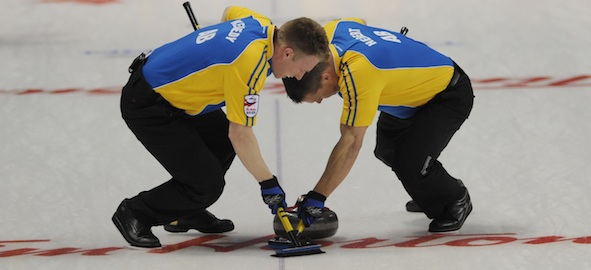
\includegraphics[width=1.0\textwidth]{Images/Sweeping.jpg}
\end{frame}

\begin{frame}\frametitle{Curling: An Introduction}
    \includemedia[
        width=1.0\textwidth,
        height=0.75\textheight,
        activate=pageopen,
        addresource=Double_for_3.mp4,
        flashvars={flv=Double_for_3.mp4&autoPlay=true}]{
            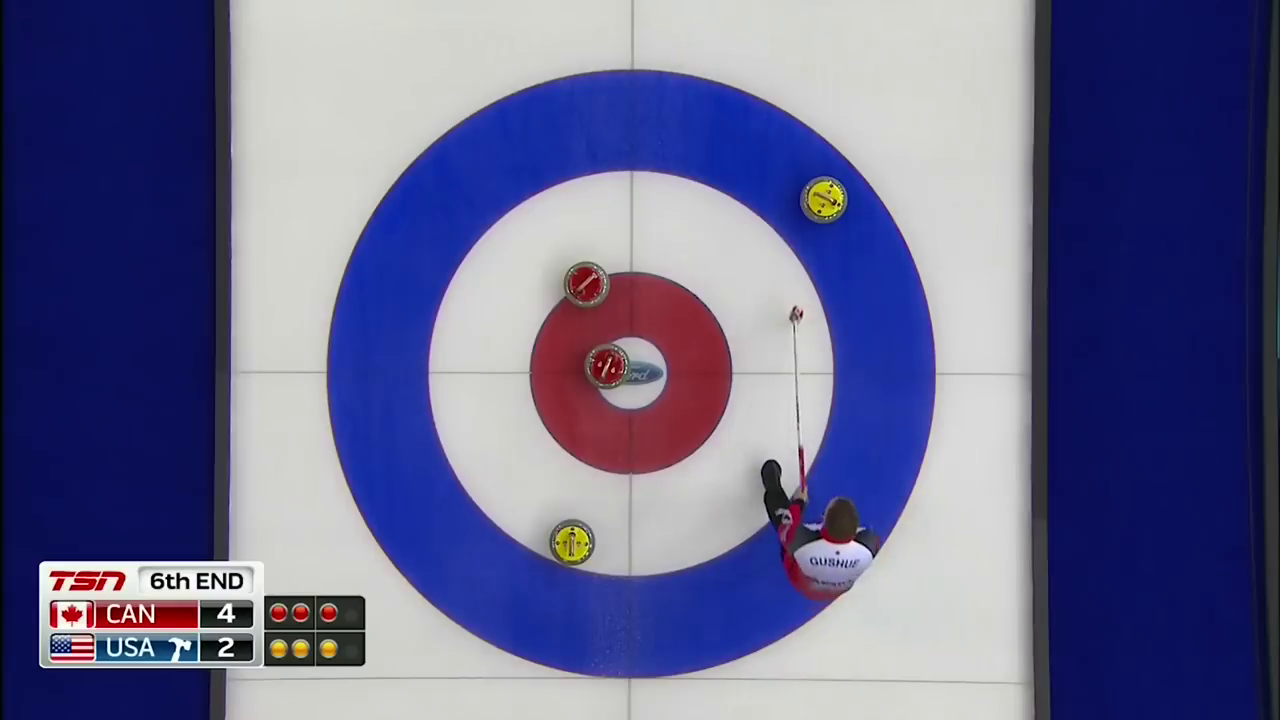
\includegraphics[width=0.8\textwidth]{Images/Double_for_3.png}
        }{player_flv_maxi.swf}
\end{frame}

\begin{frame}\frametitle{Curling: An Introduction}
    \begin{columns}
        \begin{column}{0.5\textwidth}
            \begin{block}{Curling dates back to $16^{\textnormal{th}}$ century Scotland}
                \centering
                
\includegraphics[width=0.8\textwidth]{Images/Scotland.png}
            \end{block}
        \end{column}
        \begin{column}{0.45\textwidth}
            \begin{block}{Curling was reintroduced as an Olympic sport in 1998}
                Since 1998:
                    \begin{table}
                        \centering
                        \begin{tabular}{cc}
                            Nation                                                          &Gold Medals\\
                            \hline
                            
\includegraphics[width=0.2\textwidth]{Images/Canada.png}        &5\\
                            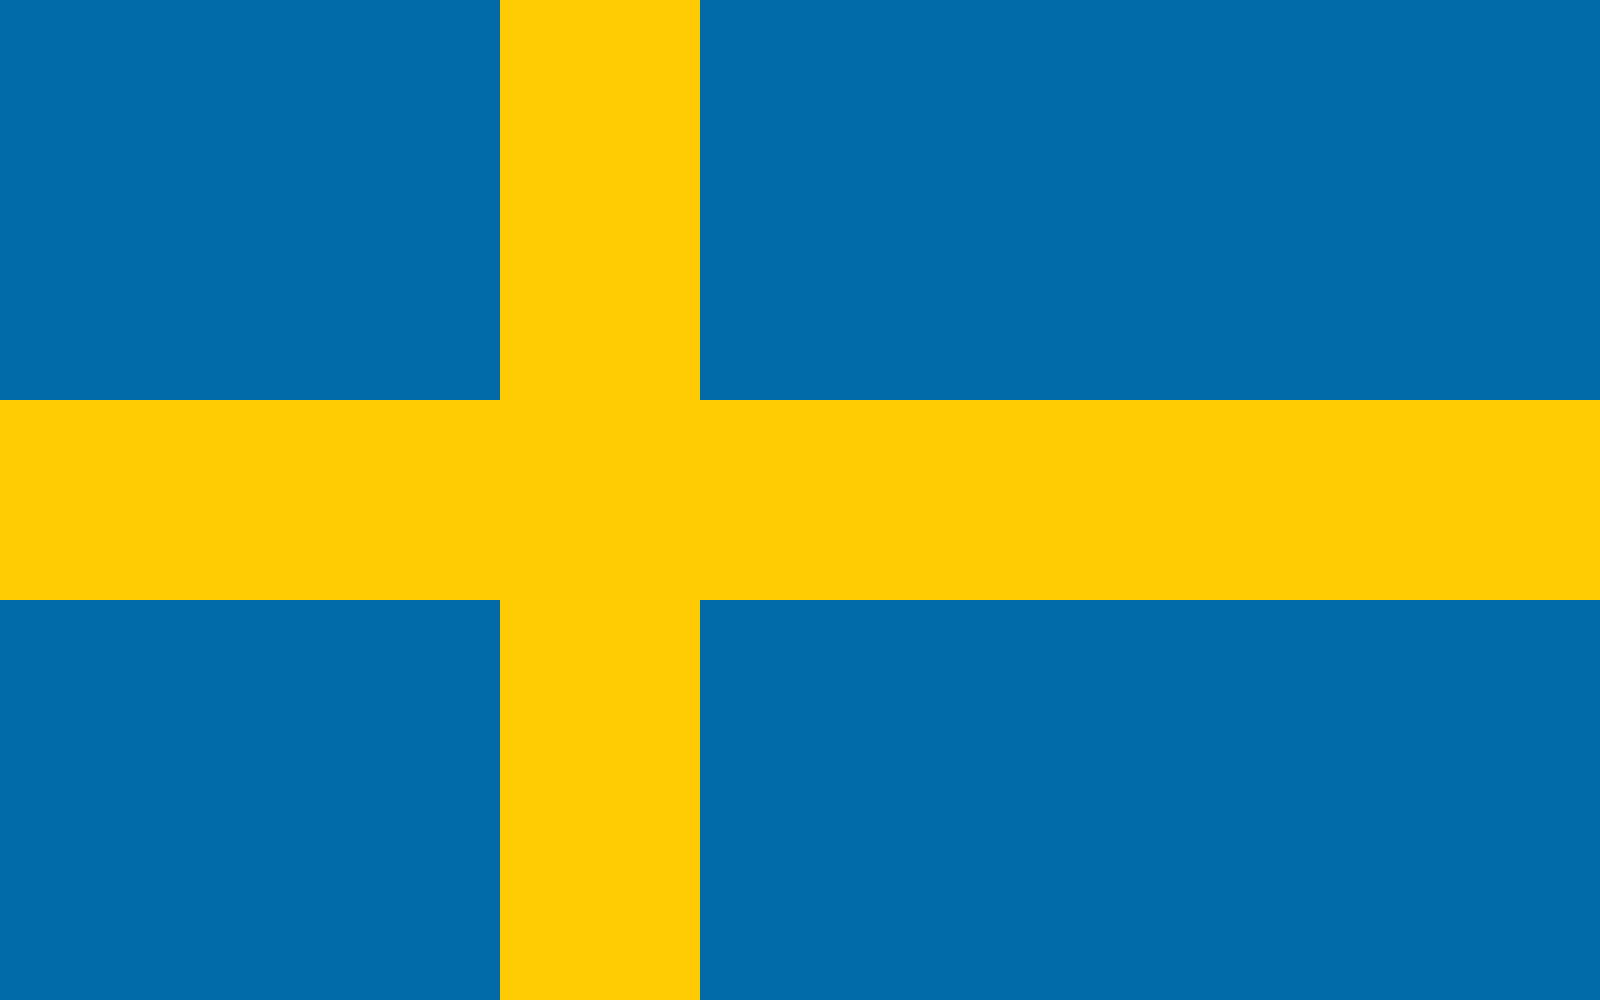
\includegraphics[width=0.2\textwidth]{Images/Sweden.png}        &2\\
                            
\includegraphics[width=0.15\textwidth]{Images/Switzerland.png}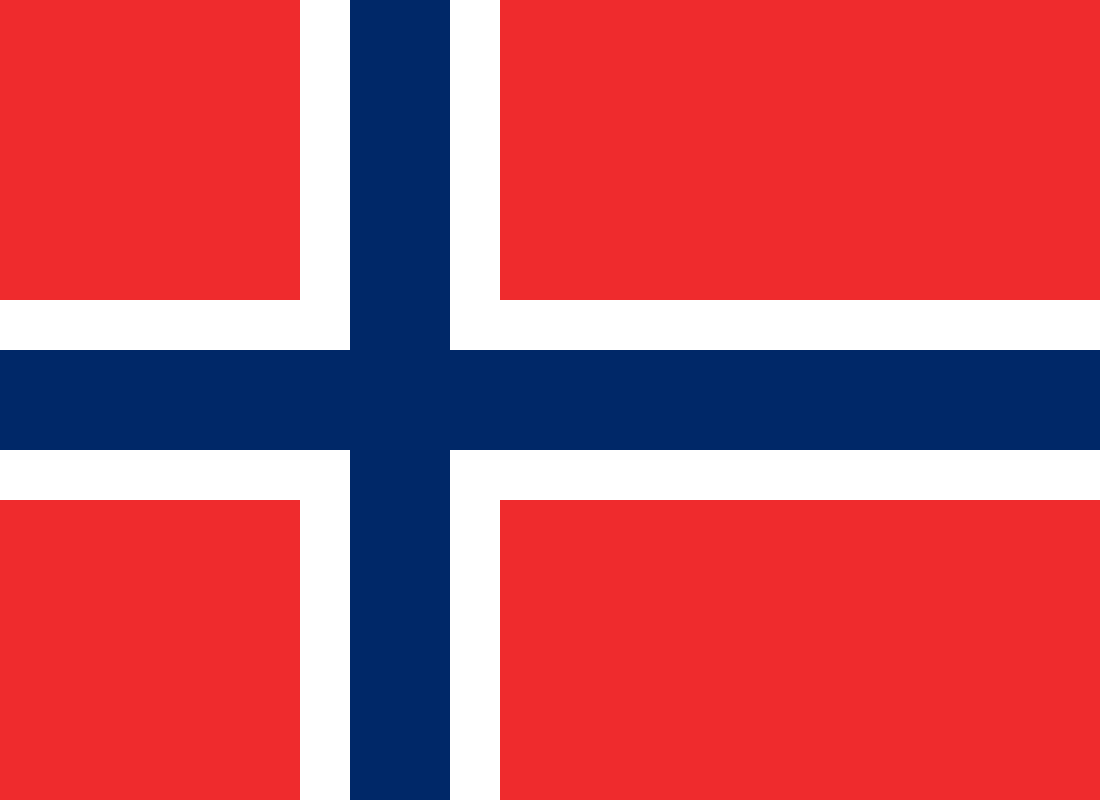
\includegraphics[width=0.15\textwidth]{Images/Norway.png}
\includegraphics[width=0.2\textwidth]{Images/UK.png}            &1\\
                        \end{tabular}
                    \end{table}
            \end{block}
        \end{column}
    \end{columns}
\end{frame}

\begin{frame}\frametitle{Curling: An Introduction}
    \begin{columns}    
        \begin{column}{0.35\textwidth}    
            \begin{itemize}
                \item The sport is played by two teams of four. 
                \item Each team takes turns sliding stones 130 feet (40 meters) toward a 12 foot (3.6 meter) target called "the house."
                \item Each team throws eight stones and are trying to get their stones as close to the center of the house this is called "the button."
            \end{itemize}
        \end{column}
        \begin{column}{0.6\textwidth}    
            \centering
            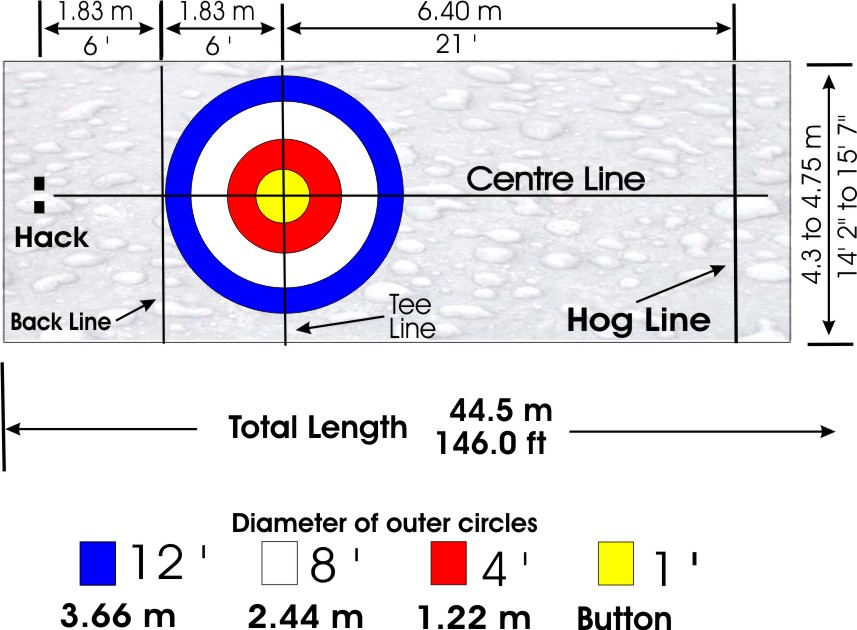
\includegraphics[width=1.0\textwidth]{Images/icesheet.jpg}
        \end{column}
    \end{columns}    
\end{frame}

\begin{frame}\frametitle{Curling: An Introduction}
    After all 16 stones are thrown the team whose rocks are closest to the button scores a point for each stone closer than their opponent's.
    \begin{block}{}
        \centering
        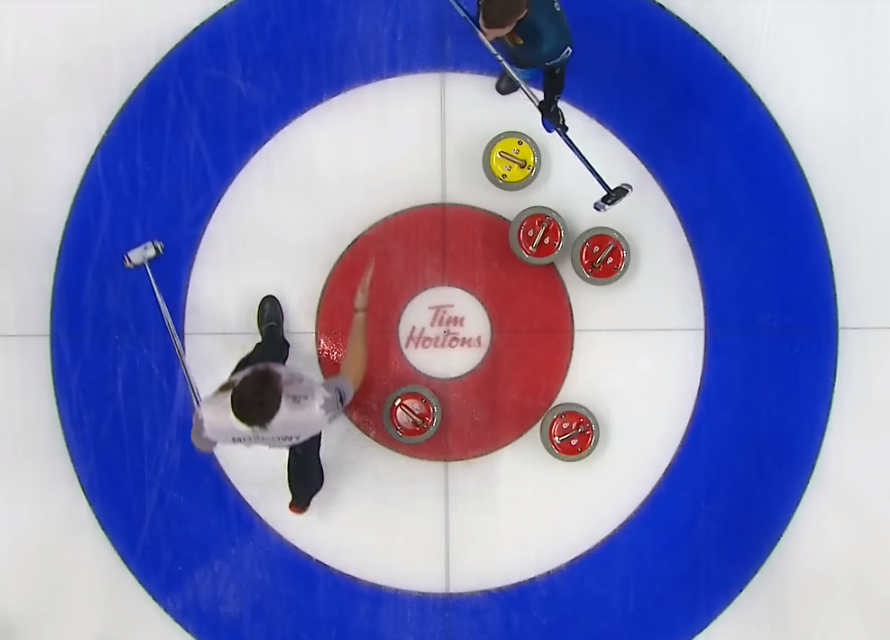
\includegraphics[width=0.7\textwidth]{Images/Score_of_4.png}\\

        Red scores four points
    \end{block}
\end{frame}

\begin{frame}\frametitle{Curling: An Introduction}
    After all 16 stones are thrown the team whose rocks are closest to the button scores a point for each stone closer than their opponent's.
    \begin{block}{}
        \centering
        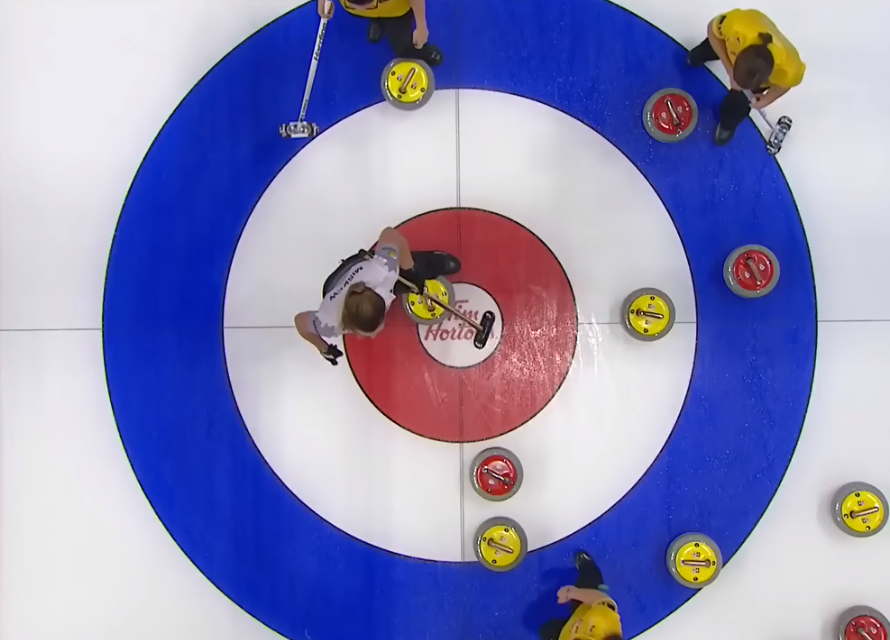
\includegraphics[width=0.7\textwidth]{Images/Score_of_1.png}\\
        Yellow scores one point
    \end{block}
\end{frame}

\begin{frame}\frametitle{Curling: An Introduction}
    \begin{columns}    
        \begin{column}{0.3\textwidth}    
            \begin{itemize}
                \item Curling stones are made of granite and weigh around 40 pounds (18 kg)
                \item The stones have concave bottoms and actually slide on a small ring
            \end{itemize}
        \end{column}
        \begin{column}{0.7\textwidth}    
            \centering
            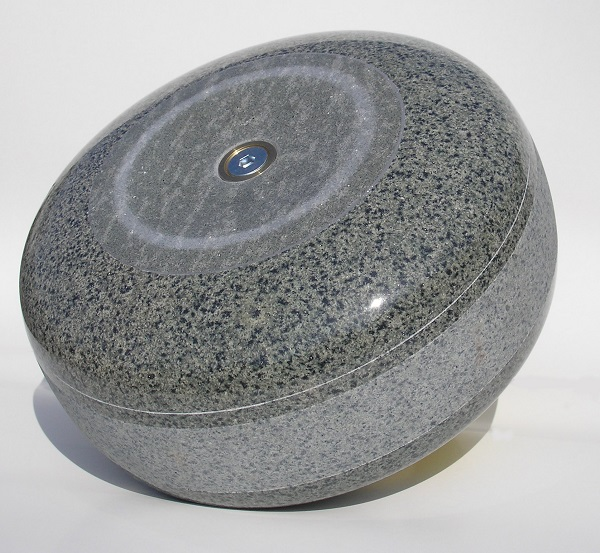
\includegraphics[width=1.0\textwidth]{Images/Curling_Stone.jpg}
        \end{column}
    \end{columns}    
\end{frame}

\begin{frame}\frametitle{Curling: An Introduction}
    \begin{columns}    
        \begin{column}{0.3\textwidth}    
            \begin{itemize}
                \item The surface of the ice is not smooth.
                \item The ice is prepared with small droplets of water frozen on the surface.
                \item This is called "the pebble"
            \end{itemize}
        \end{column}
        \begin{column}{0.7\textwidth}    
            \centering
            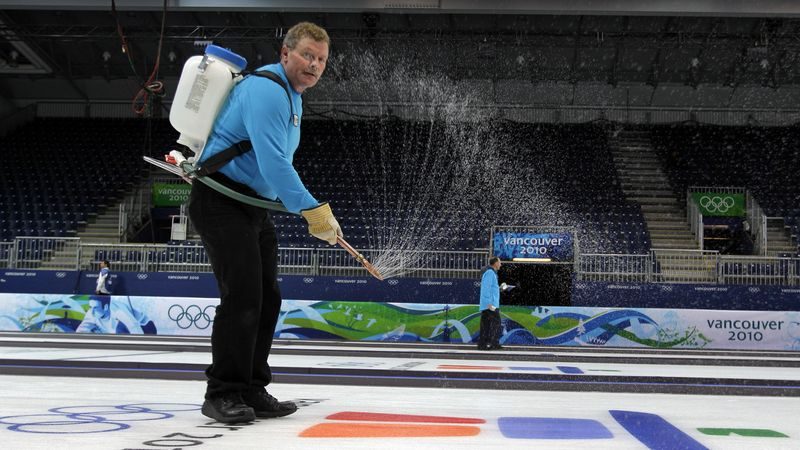
\includegraphics[width=1.0\textwidth]{Images/Pebble.jpg}
        \end{column}
    \end{columns}    
\end{frame}

\begin{frame}\frametitle{Curling: An Introduction}
    \begin{itemize}
        \item Curling gets it's name from the fact that the stones travel along curved paths
        \item This is achieved by releasing the stone with a rotation
        \item The deep and interesting strategy of the game all comes from the curling of the stones
    \end{itemize}
    \centering
    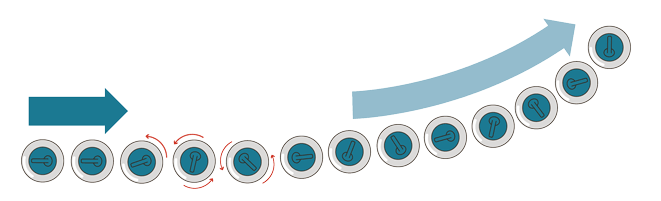
\includegraphics[width=1.0\textwidth]{Images/Curl_Path.png}
\end{frame}

\begin{frame}\frametitle{Curling: An Introduction}
    \includemedia[
        width=1.0\textwidth,
        height=0.75\textheight,
        activate=pageopen,
        addresource=Draw_Around.mp4,
        flashvars={flv=Draw_Around.mp4&autoPlay=true}]{
            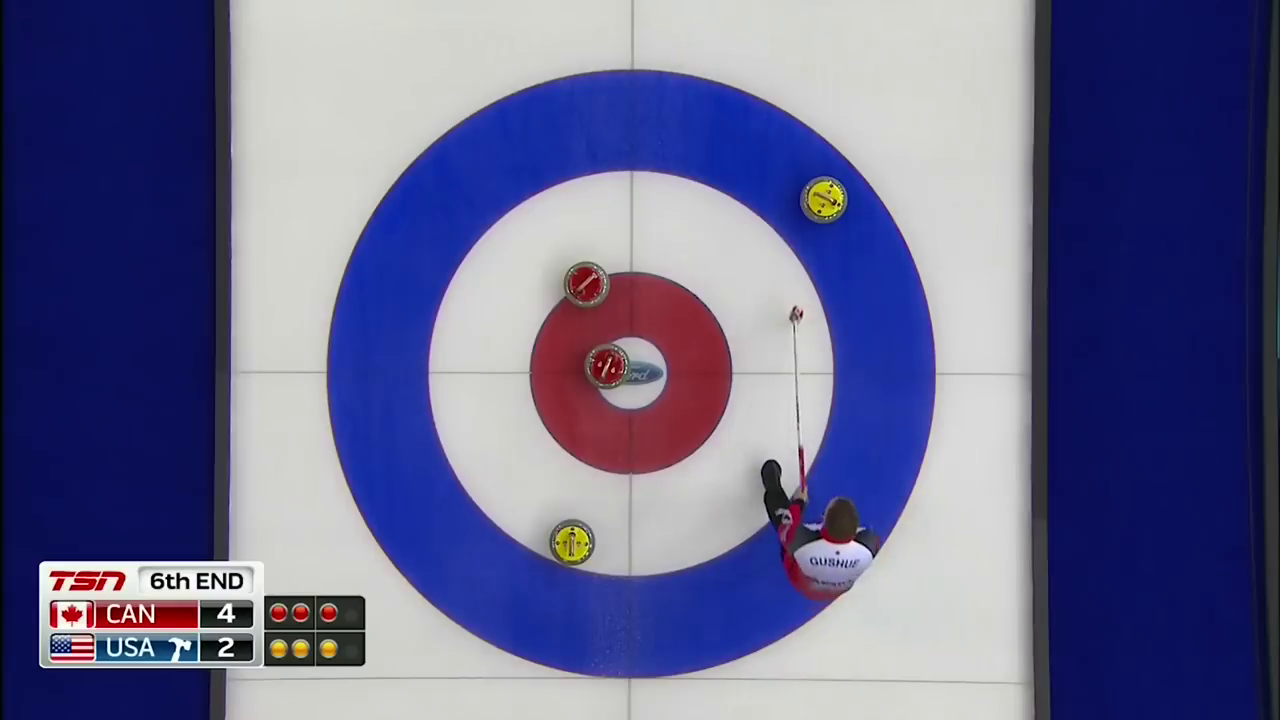
\includegraphics[width=0.8\textwidth]{Images/Double_for_3.png}
        }{player_flv_maxi.swf}
\end{frame}

\begin{frame}\frametitle{Curling: An Introduction}
    \begin{itemize}
        \item The sweeping heats the ice in front of the stone
        \item This reduces the friction on the stone
        \item This causes the stone to travel farther and straighter
    \end{itemize}
    \centering
    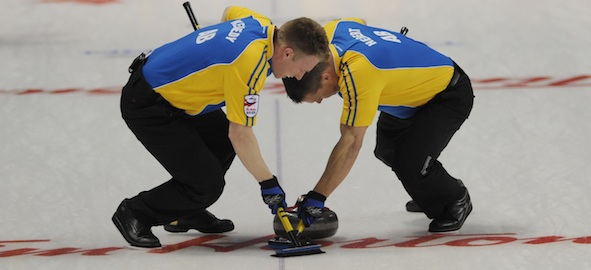
\includegraphics[width=1.0\textwidth]{Images/Sweeping.jpg}
\end{frame}


\begin{frame}\frametitle{Curling: An Introduction}
    \includemedia[
        width=1.0\textwidth,
        height=0.75\textheight,
        activate=pageopen,
        addresource=Draw_to_4ft.mp4,
        flashvars={flv=Draw_to_4ft.mp4&autoPlay=true}]{
            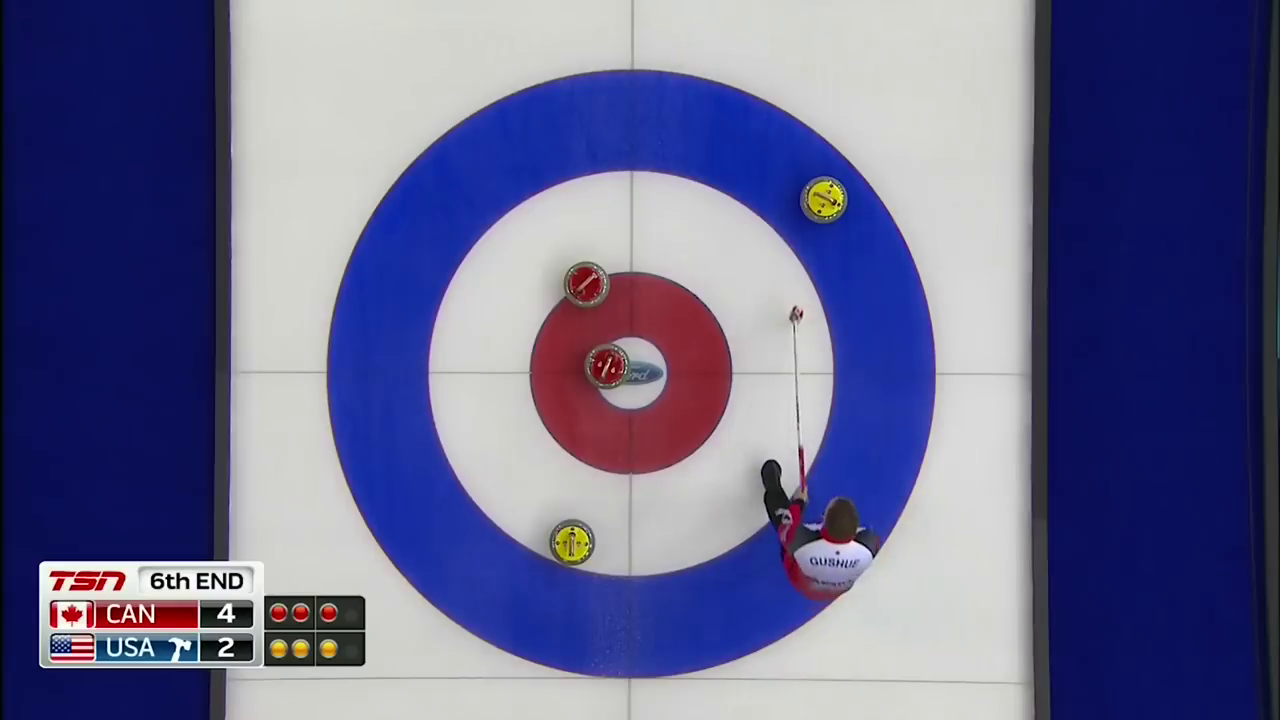
\includegraphics[width=0.8\textwidth]{Images/Double_for_3.png}
        }{player_flv_maxi.swf}
\end{frame}

\begin{frame}\frametitle{The Unintuitive Physics of the Curling Stone}
    Take for example a upside down glass rotating and sliding across a table. The glass deflects in the opposite direction than a curling stone!
    So we need a model of the curling stone that:
    \begin{itemize}
        \item Deflects in the same direction of rotation.
        \item Deflects about 1 meter when slowly rotating.
    \end{itemize}
\end{frame}

\begin{frame}\frametitle{Mark Shegelski's Model}
    \centering
    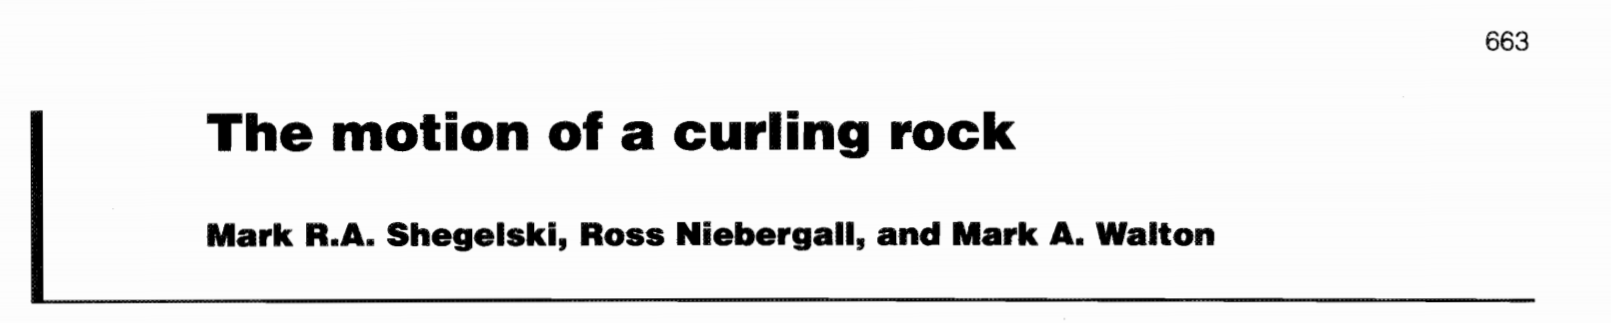
\includegraphics[width=0.9\textwidth]{Images/M_Shegelski_1996.png}

    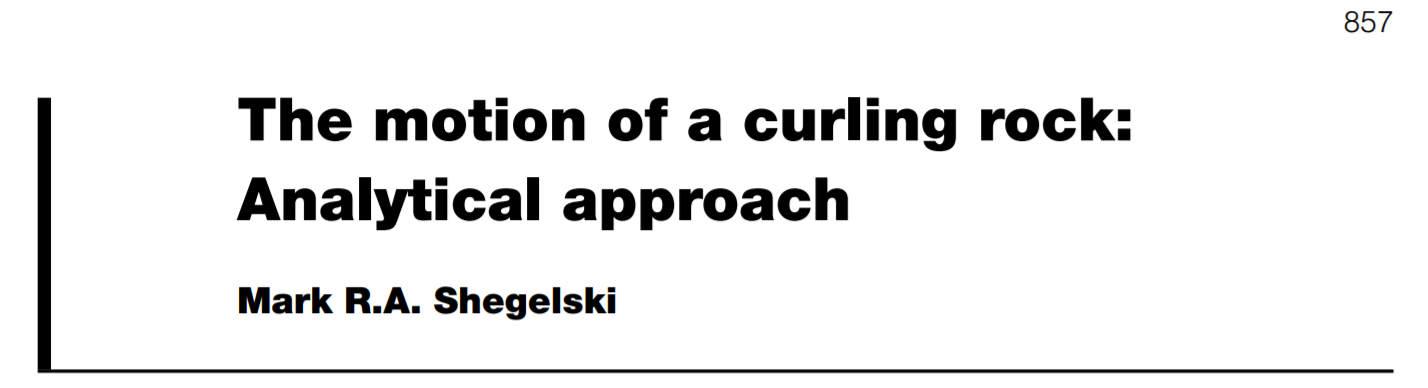
\includegraphics[width=1.0\textwidth]{Images/M_Shegelski_2000.png}

    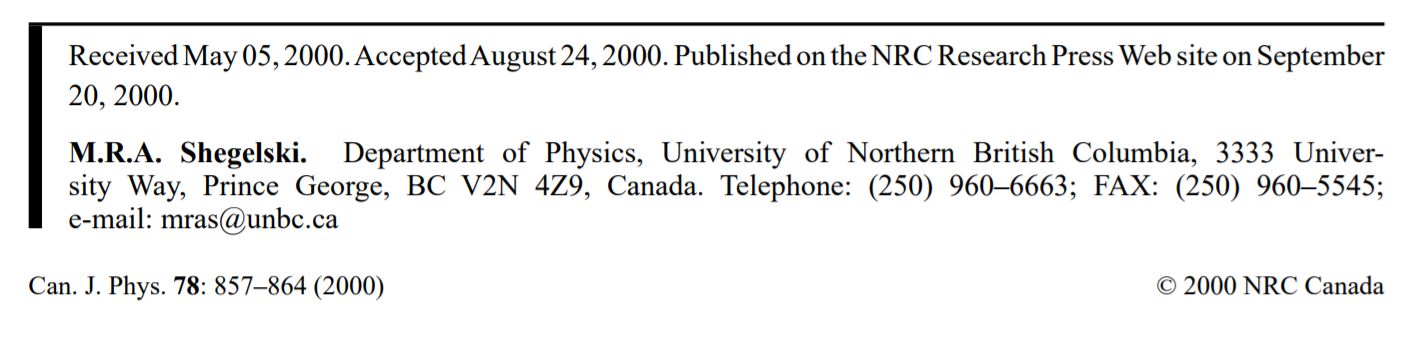
\includegraphics[width=1.0\textwidth]{Images/M_Shegelski_2000_Affl.png}
\end{frame}

\begin{frame}\frametitle{Asymmetric Friction Due to Liquid Thin Film}
    \begin{columns}    
        \begin{column}{0.6\textwidth}    
            \begin{itemize}
                \item Phase 1: The leading semicircle experiences dry friction
                \item Phase 2: The rock slows distributing the areas of wet and dry friction
                \item Phase 3: The rock moves slowly enough to drag liquid film from the back to the front creating a front back frictional asymmetry 
            \end{itemize}
            Dry friction: $\Delta{F}^{d} = \mu{M}g\left(\frac{\Delta\theta}{2\pi}\right)$ 
            Wet Friction: $\Delta{F}^{w} = k[u(\theta)]^{2}$

            \ 
            \

            \scriptsize{Can. J. Phys. Vol. 74, 1996}
        \end{column}
        \begin{column}{0.35\textwidth}    
            \centering
            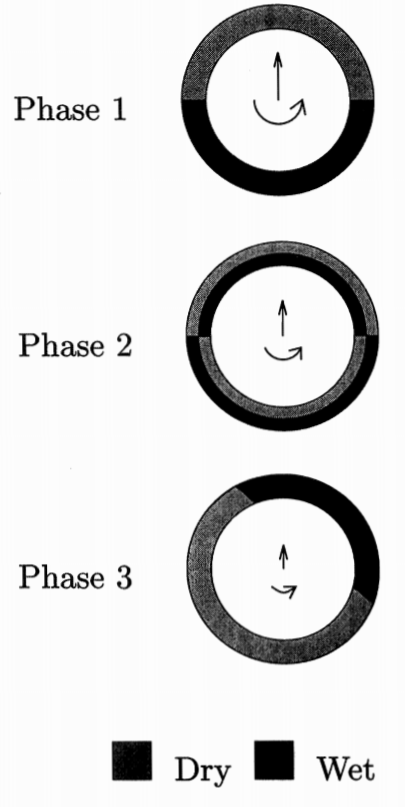
\includegraphics[width=1.0\textwidth]{Images/Wet_and_Dry.png}
        \end{column}
    \end{columns}    
\end{frame}

\begin{frame}{Front Back Frictional Asymmetry}
            \centering
            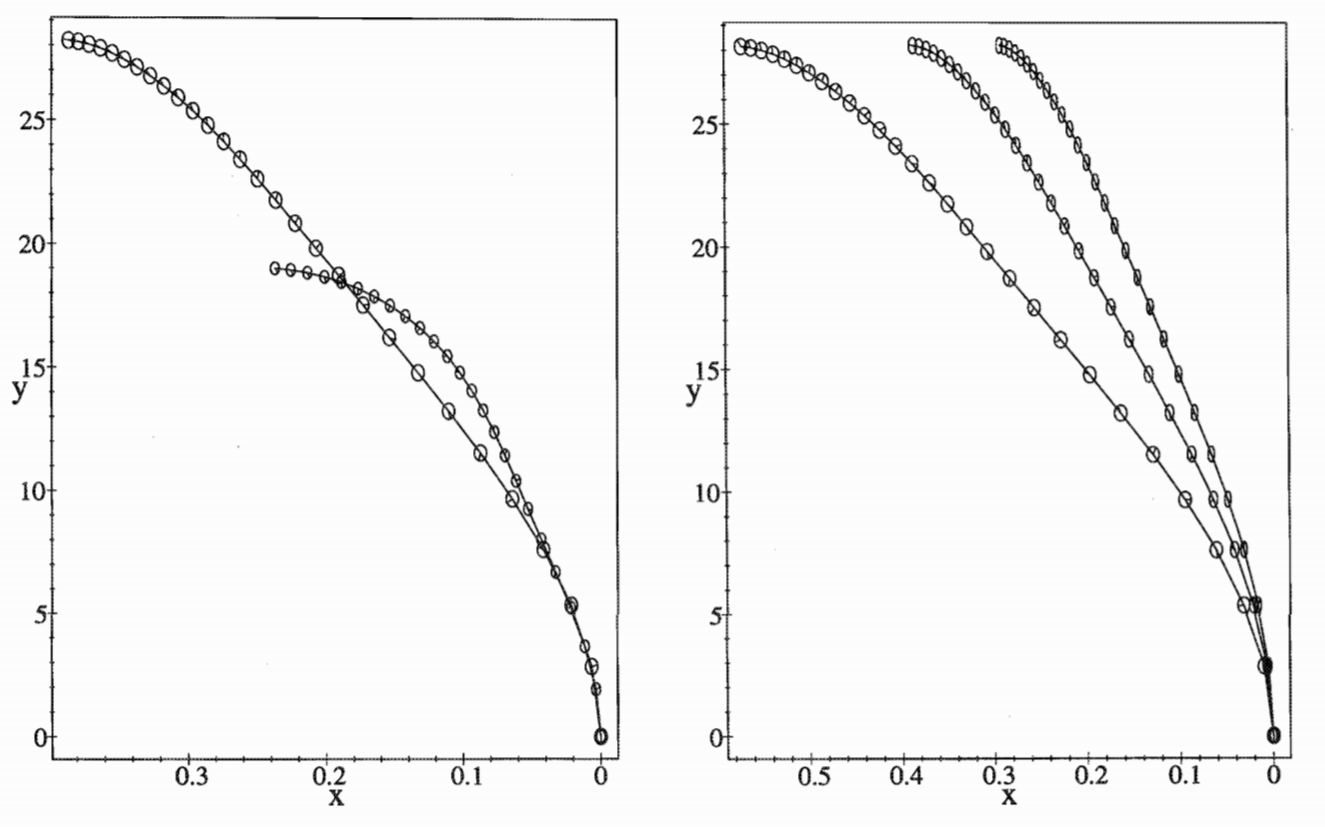
\includegraphics[width=1.0\textwidth]{Images/Shegelski_Curl_Lin_Vel.png}

            \scriptsize{Can. J. Phys. Vol. 74, 1996}
\end{frame}

\begin{frame}{Front Back Frictional Asymmetry}
    The model was simplified using the assumption that the coefficient of kinetic friction felt by the running band of the stone went by
    $$\mu(\theta) = \mu_0(1-f_0\sin\theta)$$
    The resulting force and dynamics give the desired deflection seen by curling stones

    \centering
    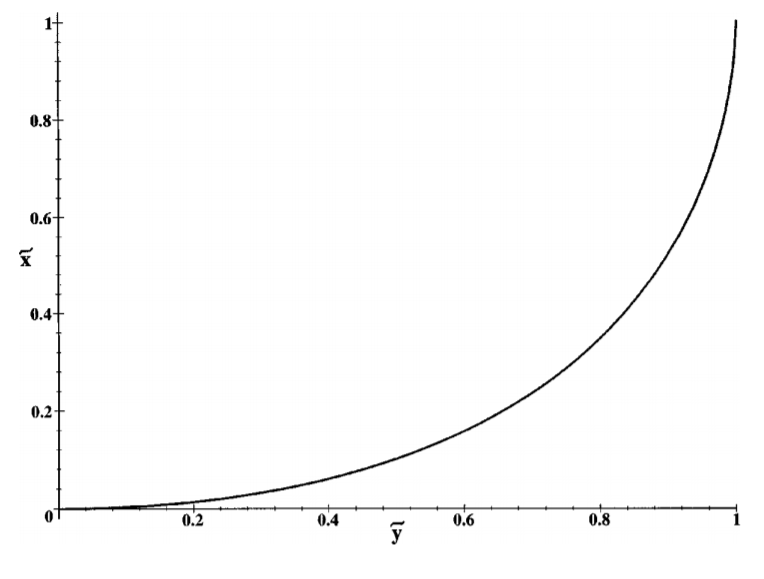
\includegraphics[width=0.5\textwidth]{Images/Shegelski_Curl_Fig.png}

    \scriptsize{Can. J. Phys. Vol. 78, 2000}
\end{frame}

\begin{frame}\frametitle{Mark Denny's Model}
    \centering
    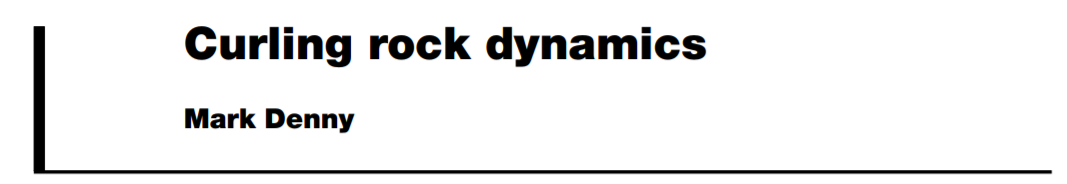
\includegraphics[width=1.0\textwidth]{Images/M_Denny_1998.png}

    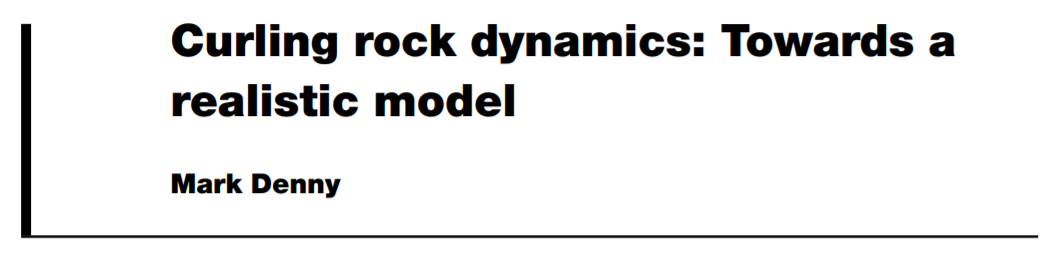
\includegraphics[width=1.0\textwidth]{Images/M_Denny_2003.png}

    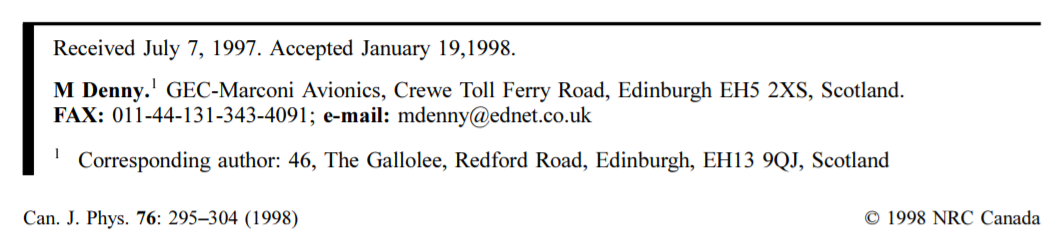
\includegraphics[width=1.0\textwidth]{Images/M_Denny_1998_Affl.png}
\end{frame}

\begin{frame}{Left Right Frictional Asymmetry}
    Denny showed that with a left right asymmetric $\mu_k$ independent of velocity the desired curl path can be achieved
    \begin{center}
    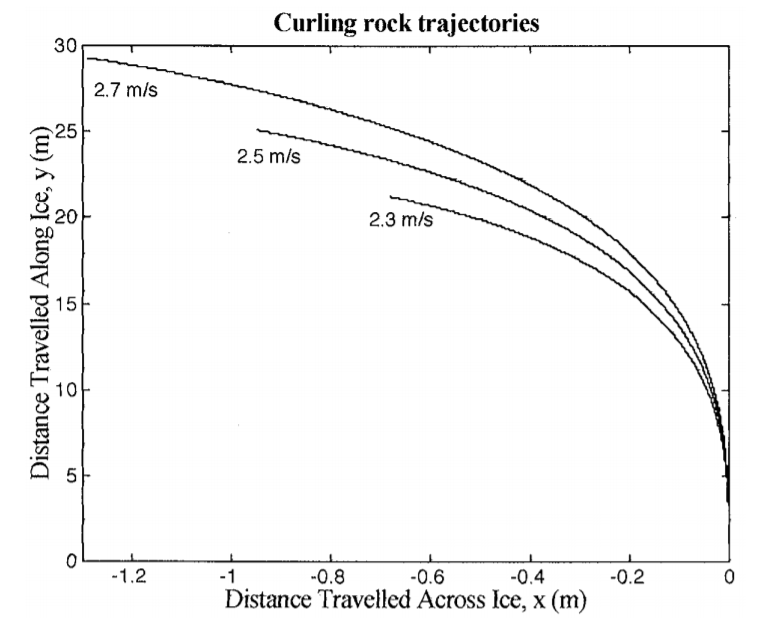
\includegraphics[width=0.7\textwidth]{Images/Denny_Traj.png}

    \scriptsize{Can. J. Phys. Vol. 78, 2000}
    \end{center}
\end{frame}

\begin{frame}{Snowplow Model}
    Denny proposed that as the stone rotates it picks up pieces of ice thereby reducing the fiction of the running band resulting in an asymmetric friction
    \begin{center}
    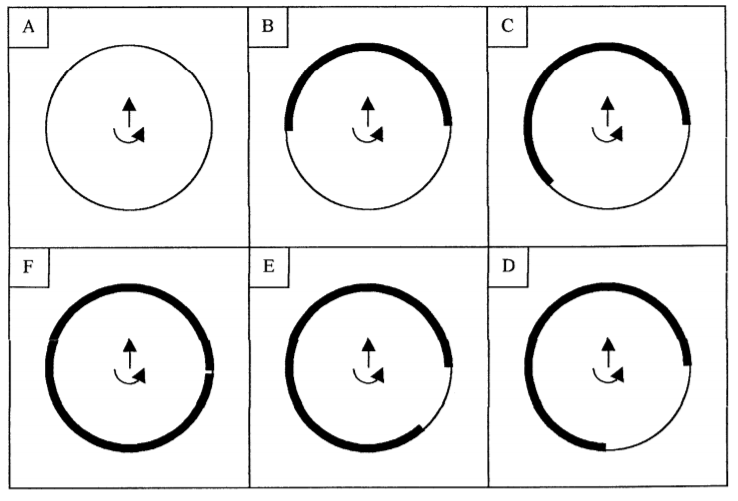
\includegraphics[width=0.7\textwidth]{Images/Snowplow.png}

    \scriptsize{Can. J. Phys. Vol. 80, 2002}
    \end{center}
\end{frame}

\begin{frame}{Criticism of Shegelski's Model}
    \begin{center}
        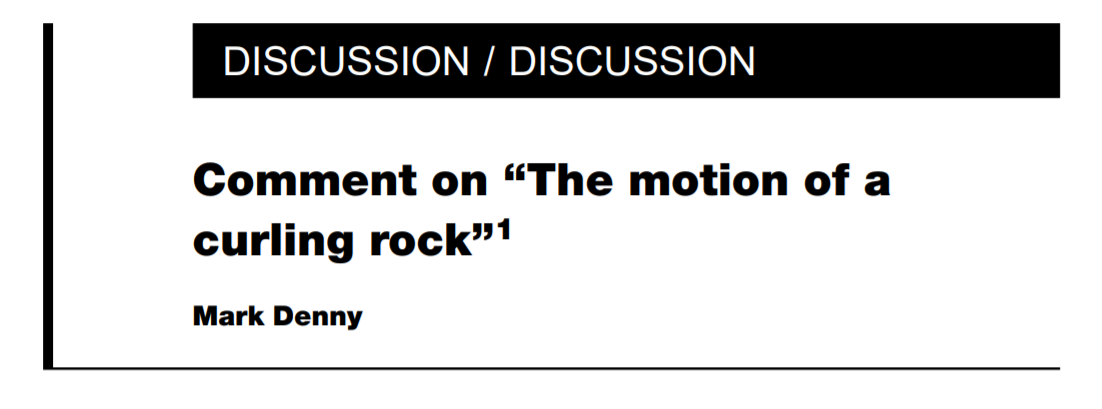
\includegraphics[width=0.55\textwidth]{Images/Denny_Comment.png}
    \end{center}
    \begin{columns}
        \begin{column}{0.4\textwidth}
            M. Denny's comment brings up two criticisms Shegelski's Model
            \begin{itemize}
                \item The number of rotations $N$ is independent of total travel time $t_0$
                \item The dependence of deflection distance on initial angular velocity does not agree with observation.
            \end{itemize}

        \end{column}
        \begin{column}{0.59\textwidth}
            \begin{center}
                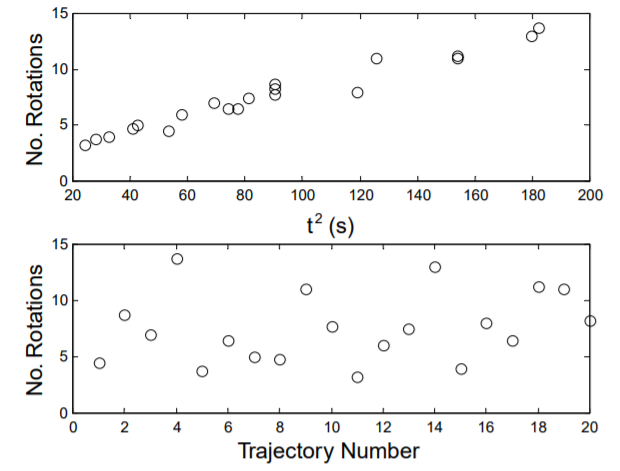
\includegraphics[width=1.0\textwidth]{Images/Denny_Comment_Plot.png}
            \end{center}
        \end{column}
    \end{columns}
\end{frame}

\begin{frame}{Response by Shegelski}
    \begin{center}
        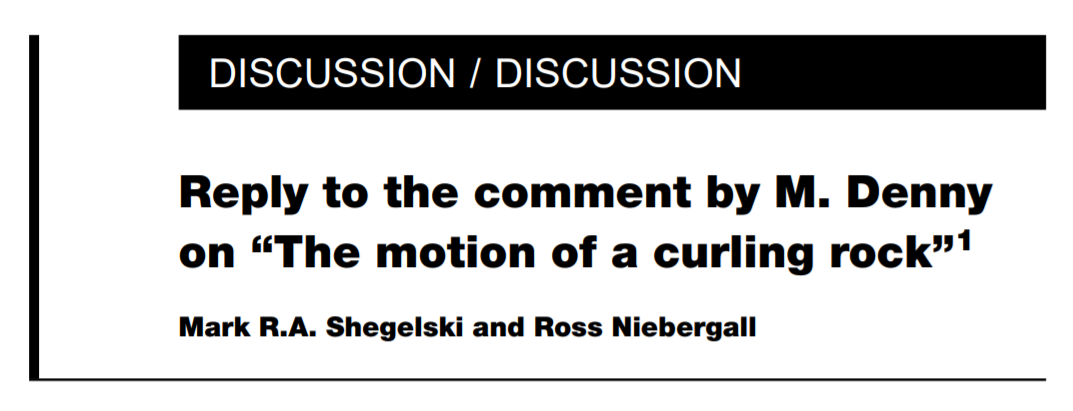
\includegraphics[width=0.55\textwidth]{Images/Denny_Comment_Reply.png}
    \end{center}
    \begin{columns}
        \begin{column}{0.4\textwidth}
            Shegelski preformed his own experiment determining the relationship between rotations $N_{Tot}$ and total time $t_{Tot}$. He fits his data to 
            $$N_{Tot} = m(t_{Tot})^{p}$$
            to find that $p=1.637\pm0.024$ which implies wet friction.
        \end{column}
        \begin{column}{0.59\textwidth}
            \begin{center}
                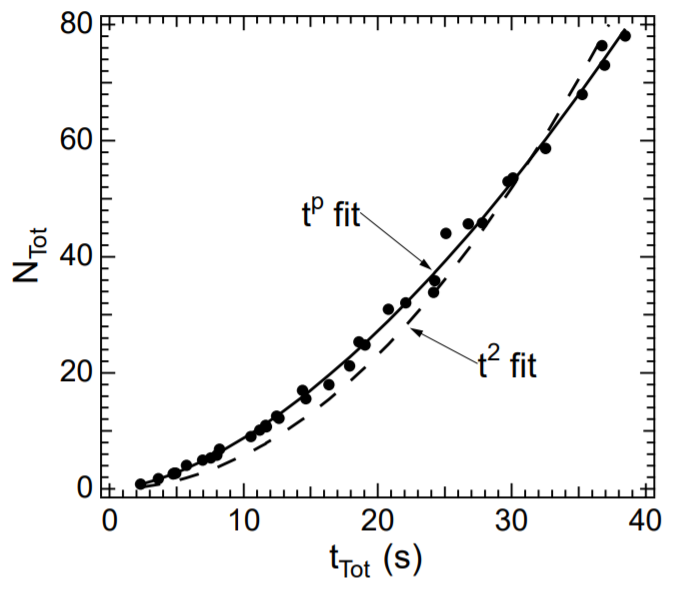
\includegraphics[width=0.88\textwidth]{Images/Denny_Comment_Reply_Plot.png}
            \end{center}
        \end{column}
    \end{columns}
\end{frame}
    
\begin{frame}\frametitle{A. Raymond Penner's Model}
    \begin{center}
    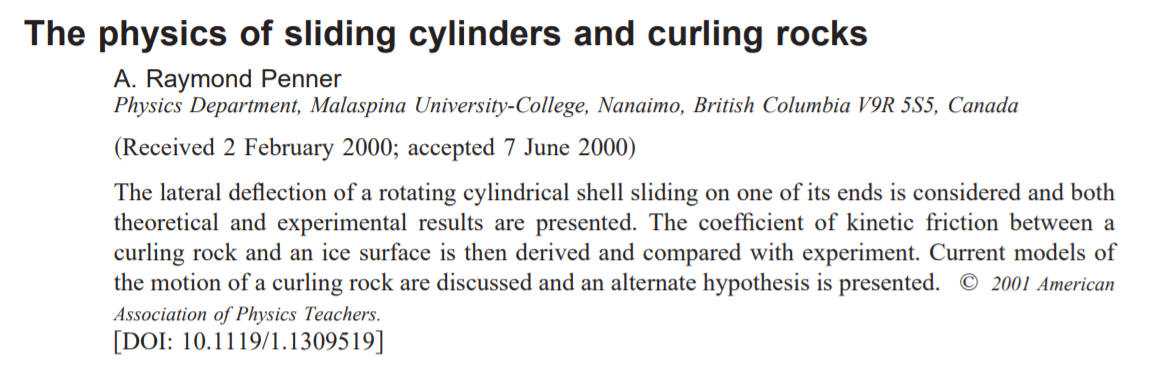
\includegraphics[width=1.0\textwidth]{Images/A_Penner_2000.png}
    \end{center}
\end{frame}

\begin{frame}\frametitle{A. Raymond Penner's Model}
    \begin{columns}
        \begin{column}{0.3\textwidth}
            A. R. Penner showed that if the frictional energy is conducted into the ice the resulting coefficient of friction goes by
            $$\mu_k \propto v^{-1/2}$$
        \end{column}
        \begin{column}{0.7\textwidth}
            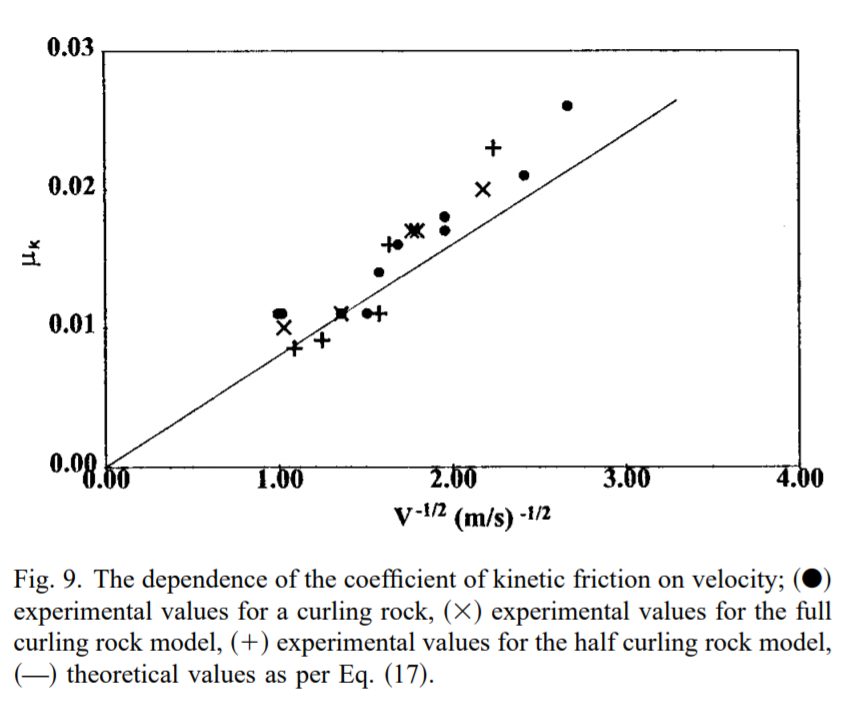
\includegraphics[width=1.0\textwidth]{Images/Mu_vs_V.png}

            \scriptsize{Am. J. Phys. Vol. 69, No. 3, March 2001}
        \end{column}
    \end{columns}
\end{frame}

\begin{frame}\frametitle{A. Raymond Penner's Model}
    \centering
    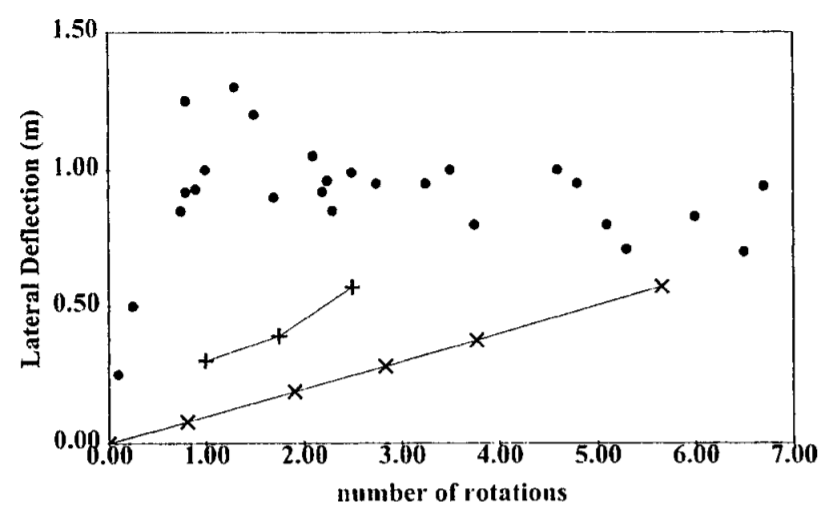
\includegraphics[width=0.8\textwidth]{Images/Deflection_vs_Angvel.png}

    \scriptsize{Am. J. Phys. Vol. 69, No. 3, March 2001}
\end{frame}

\begin{frame}\frametitle{Harald Nyberg Model}
    \centering
    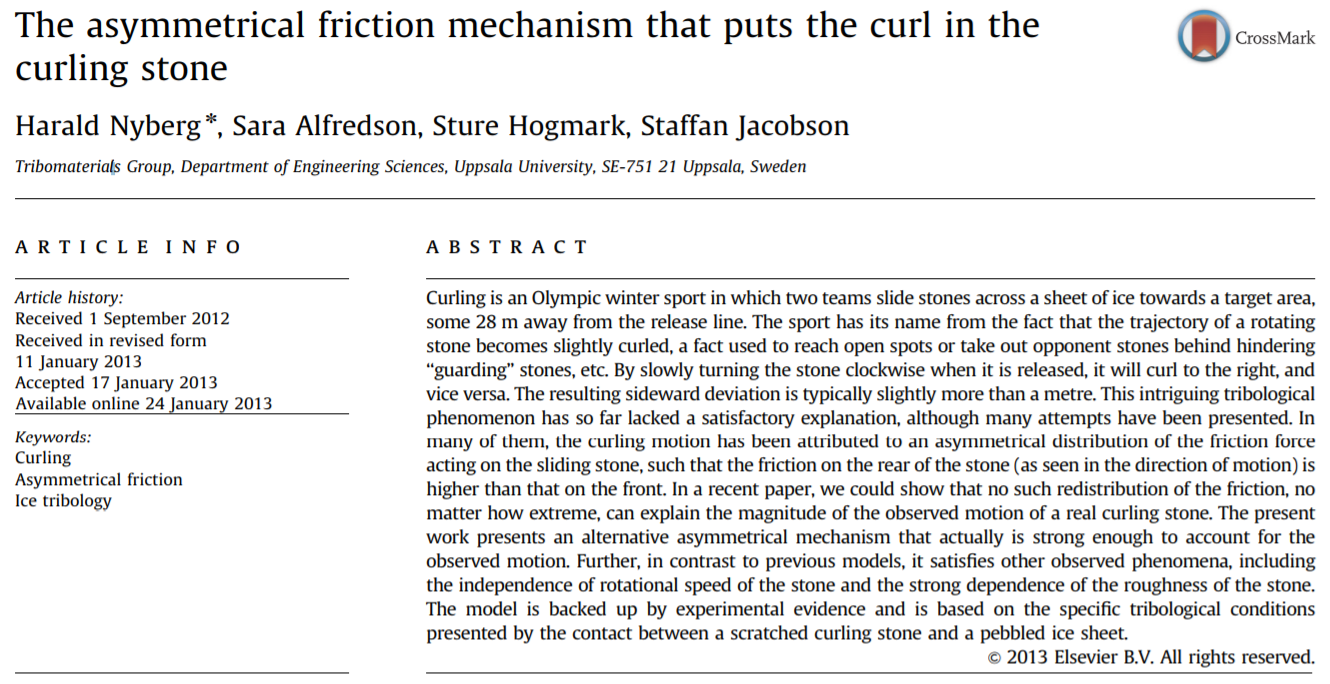
\includegraphics[width=1.0\textwidth]{Images/Nyberg_Title.png}
\end{frame}

\begin{frame}\frametitle{Harald Nyberg Model}
    Nyberg proposed that the asymmetric friction is a result of the curling stone scratching the ice.
    \centering
    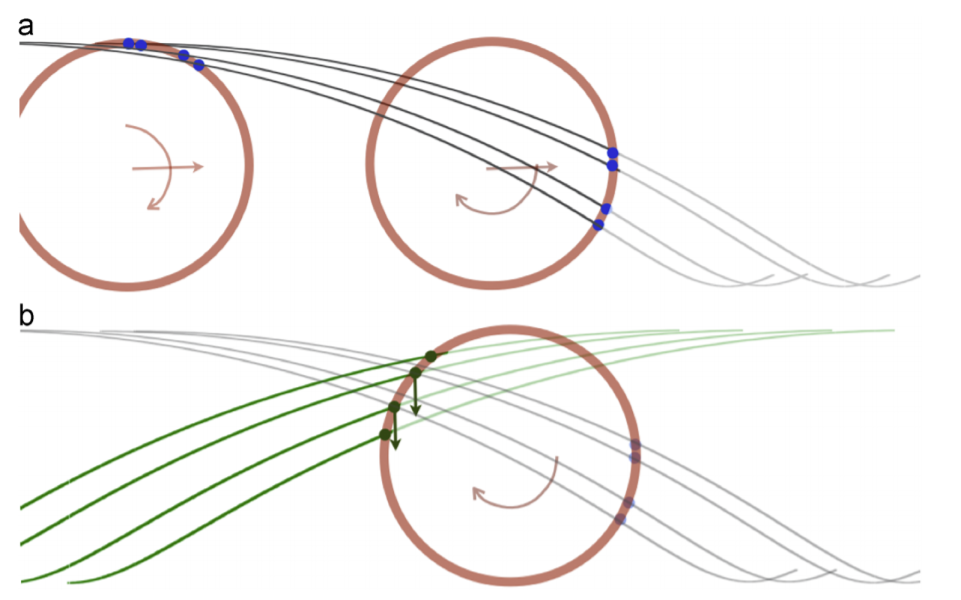
\includegraphics[width=0.8\textwidth]{Images/Scratch_Fig.png}

    \scriptsize{Wear 301 (2013) 583-589}
\end{frame}

\begin{frame}\frametitle{Harald Nyberg Model}
    Nyberg observed scratches on the pebble after a single stone has passed. As well as a change in coefficient of friction by manually scratching the ice.
    \centering
    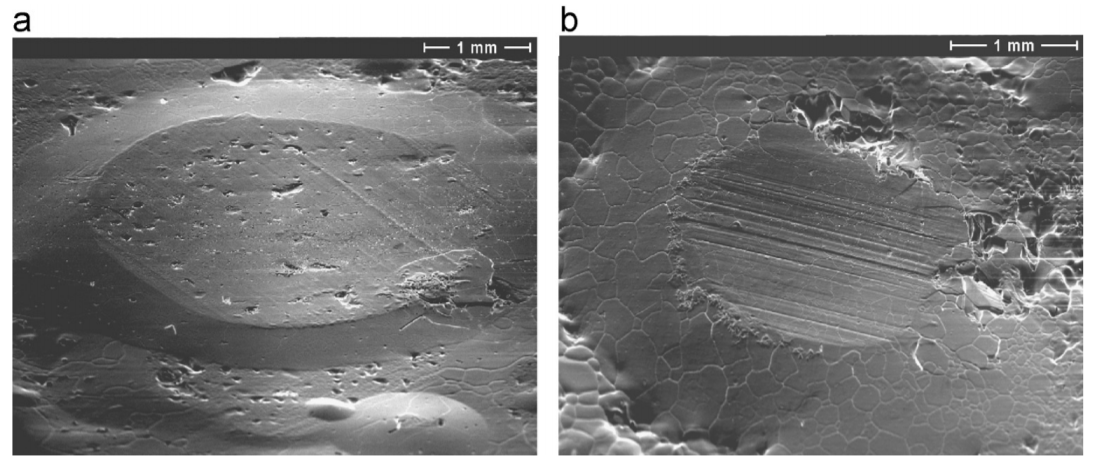
\includegraphics[width=0.8\textwidth]{Images/Scratch_SEM.png}

    \scriptsize{Wear 301 (2013) 583-589}
\end{frame}

\begin{frame}\frametitle{Shegelski Comments on the Harald Nyberg Model}
    \begin{center}
    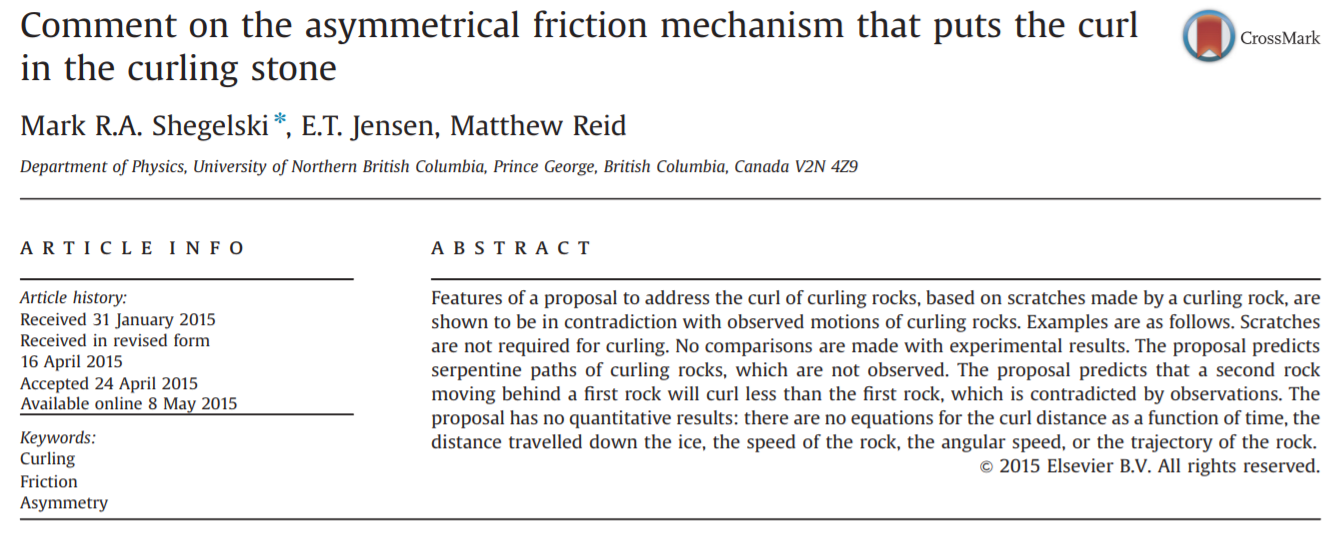
\includegraphics[width=1.0\textwidth]{Images/Nyberg_Comment.png}
    \end{center}
    Shegelski has two main complaints of the scratch model:
    \begin{itemize}
        \item The model predicts oscillations in the path and this is not observed behavior
        \item Even with a polished running surface that does not scratch the ice a curved path is observed
    \end{itemize}
\end{frame}

\begin{frame}\frametitle{Numerical Calculations of Asymmetrical Friction}
    \centering
    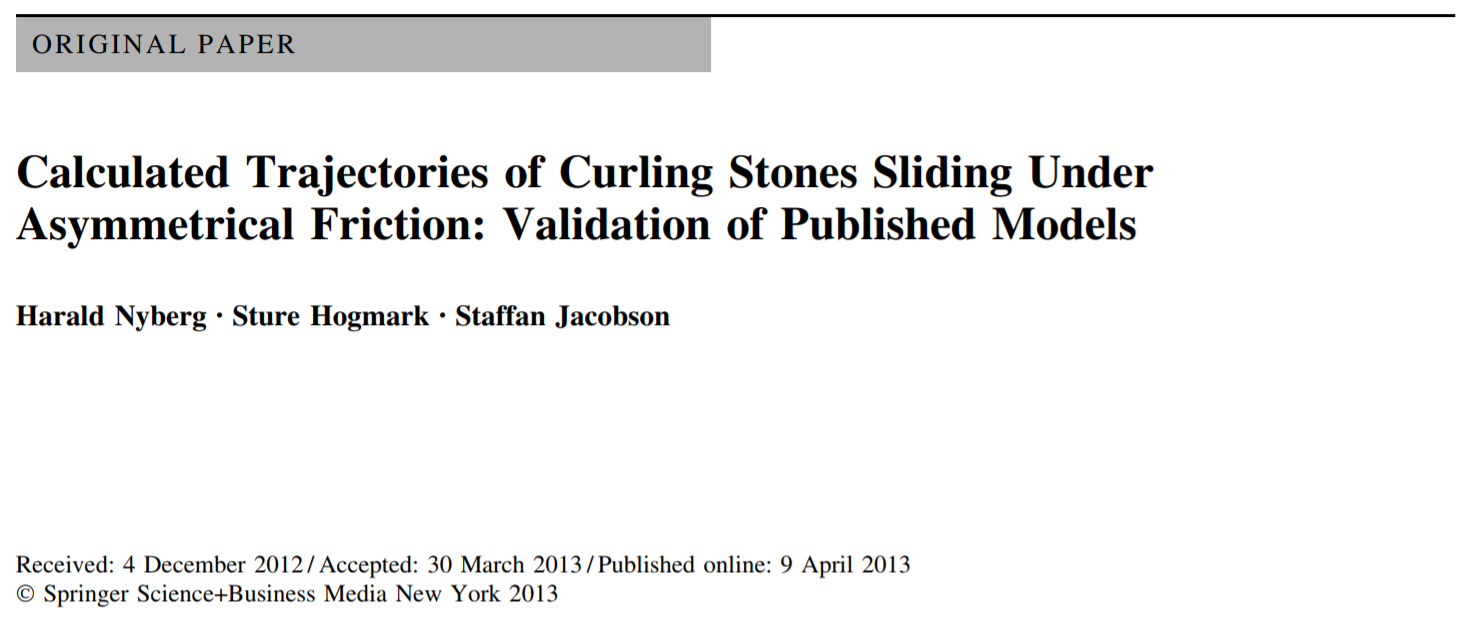
\includegraphics[width=1.0\textwidth]{Images/Nyberg_Title_2013.png}
\end{frame}

\begin{frame}\frametitle{Numerical Calculations of Asymmetrical Friction}
    Nyberg created a numerical simulation with the ability vary asymmetrical friction in a rotating cylinder. The resulting deflections are well short of observed curling stone deflections even in extreme cases.
    \centering
    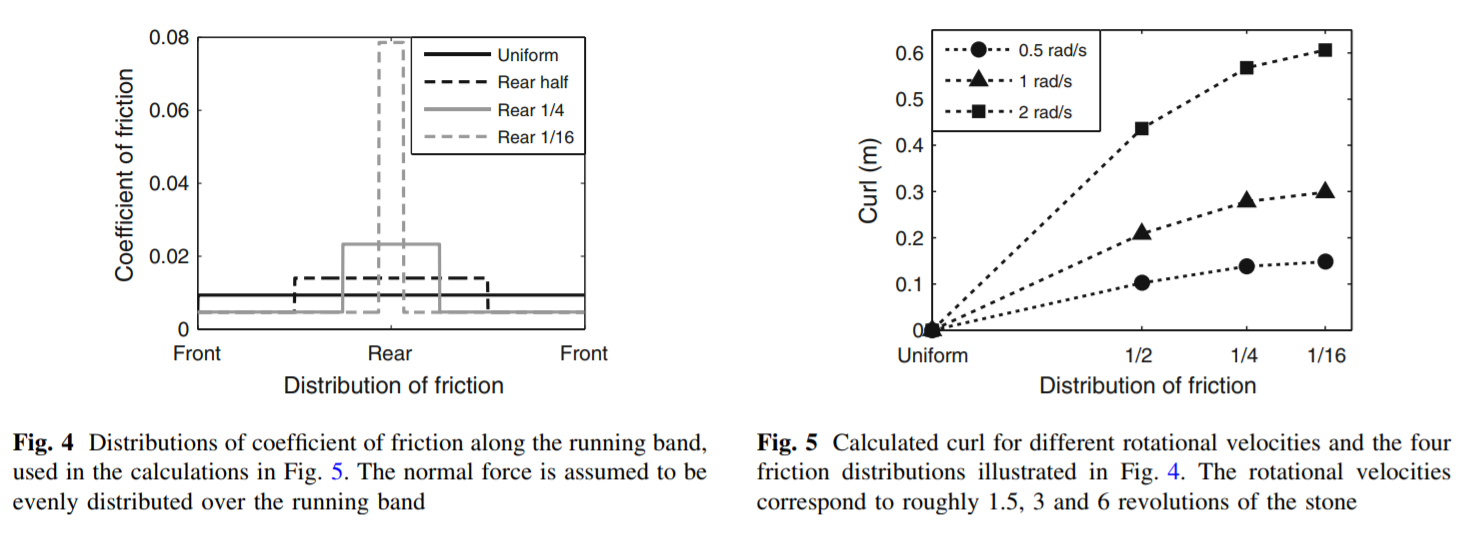
\includegraphics[width=1.0\textwidth]{Images/Numerical_Fric.png}
\end{frame}

\begin{frame}\frametitle{Further Precision Measurements}
    Measurements show as rotational speed increases deflection decreases.
    \centering
    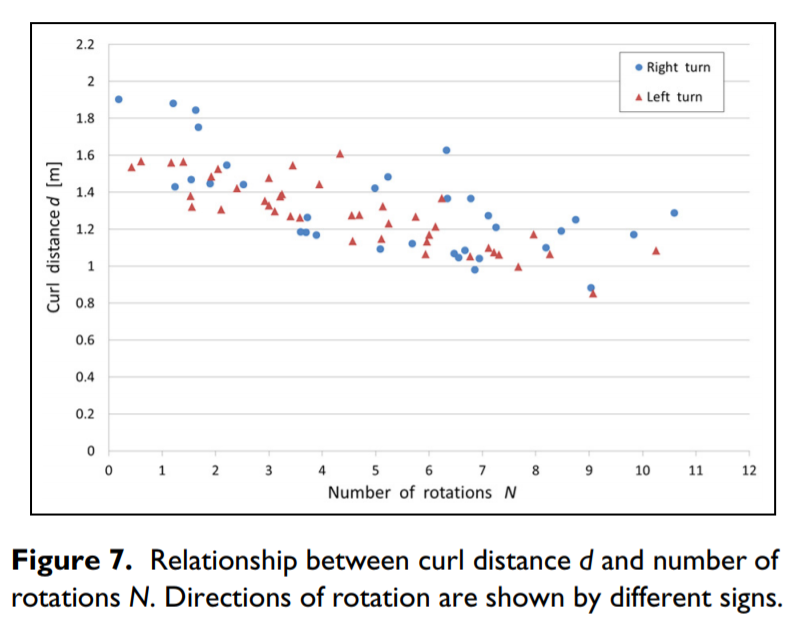
\includegraphics[width=0.7\textwidth]{Images/Precision_Mes.png}

    \scriptsize{Hattori et al. (2016)}
\end{frame}

\begin{frame}\frametitle{Pivot-Slide Model}
    \centering
    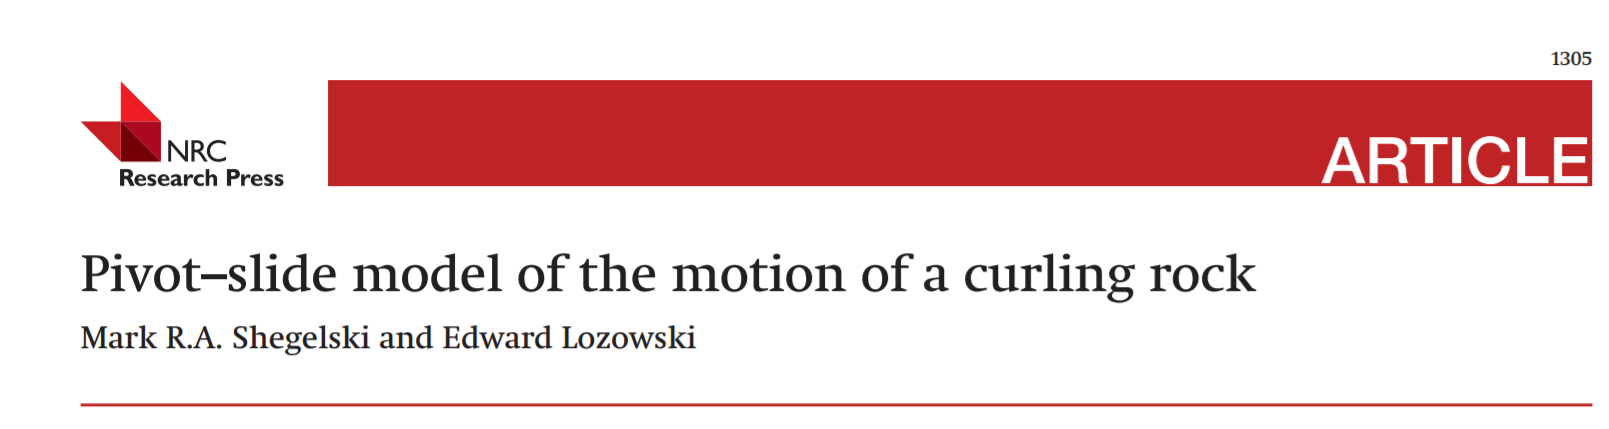
\includegraphics[width=1.0\textwidth]{Images/Pivot_Title_2016.png}

    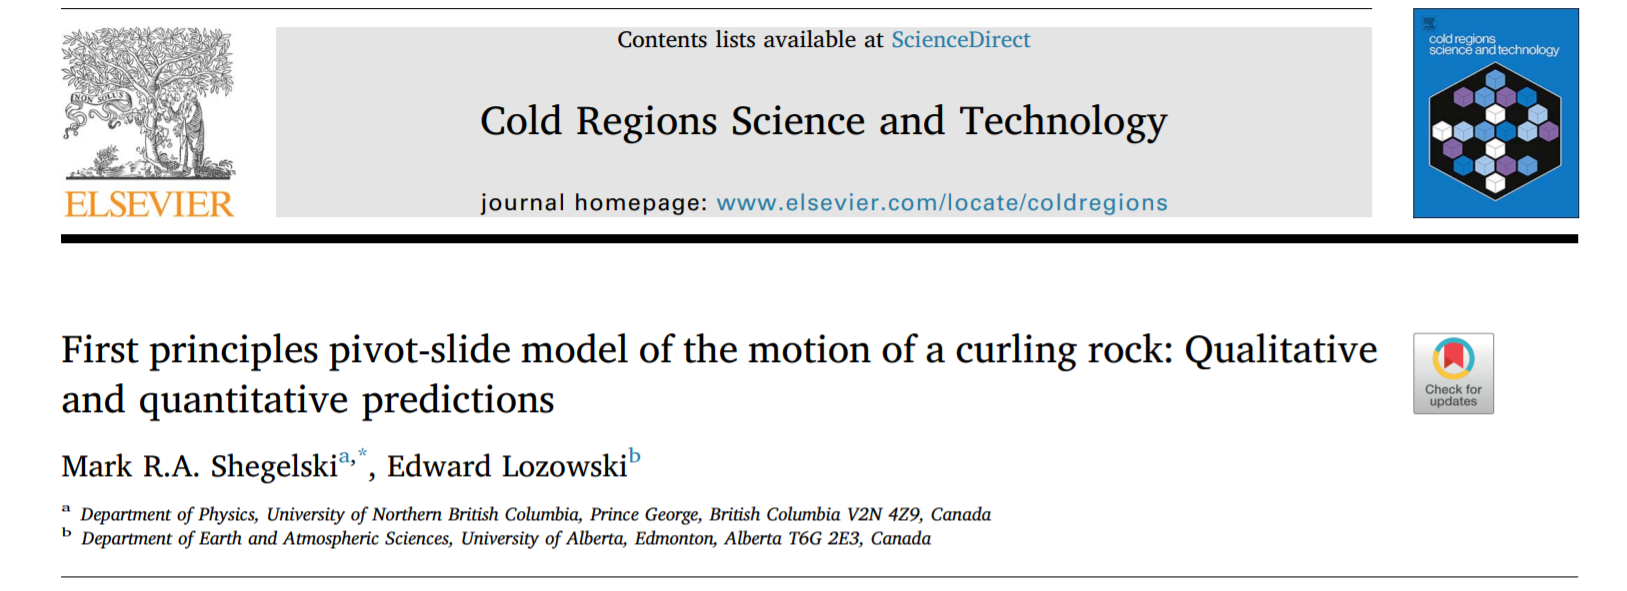
\includegraphics[width=1.0\textwidth]{Images/Pivot_Title_2018.png}
\end{frame}

\begin{frame}\frametitle{Pivot-Slide Model}
    The pivot-slide model proposes that the curl results from an adhesion of the running band with the pebbled ice. The major advantage of this model is that the deflection distance is weakly dependent on the angular velocity.
    \centering
    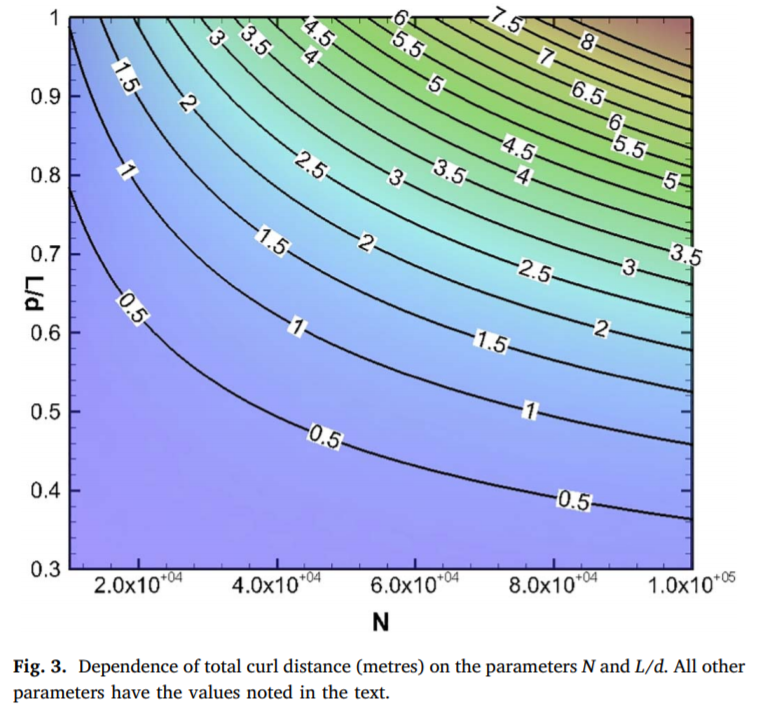
\includegraphics[width=0.7\textwidth]{Images/Pivot_Fig.png}
    \scriptsize{Cold Regions Science and Technology 146 (2018) 182-186}
\end{frame}

\begin{frame}{The Olympic Curling Competition Starts February 14}
    \centering
    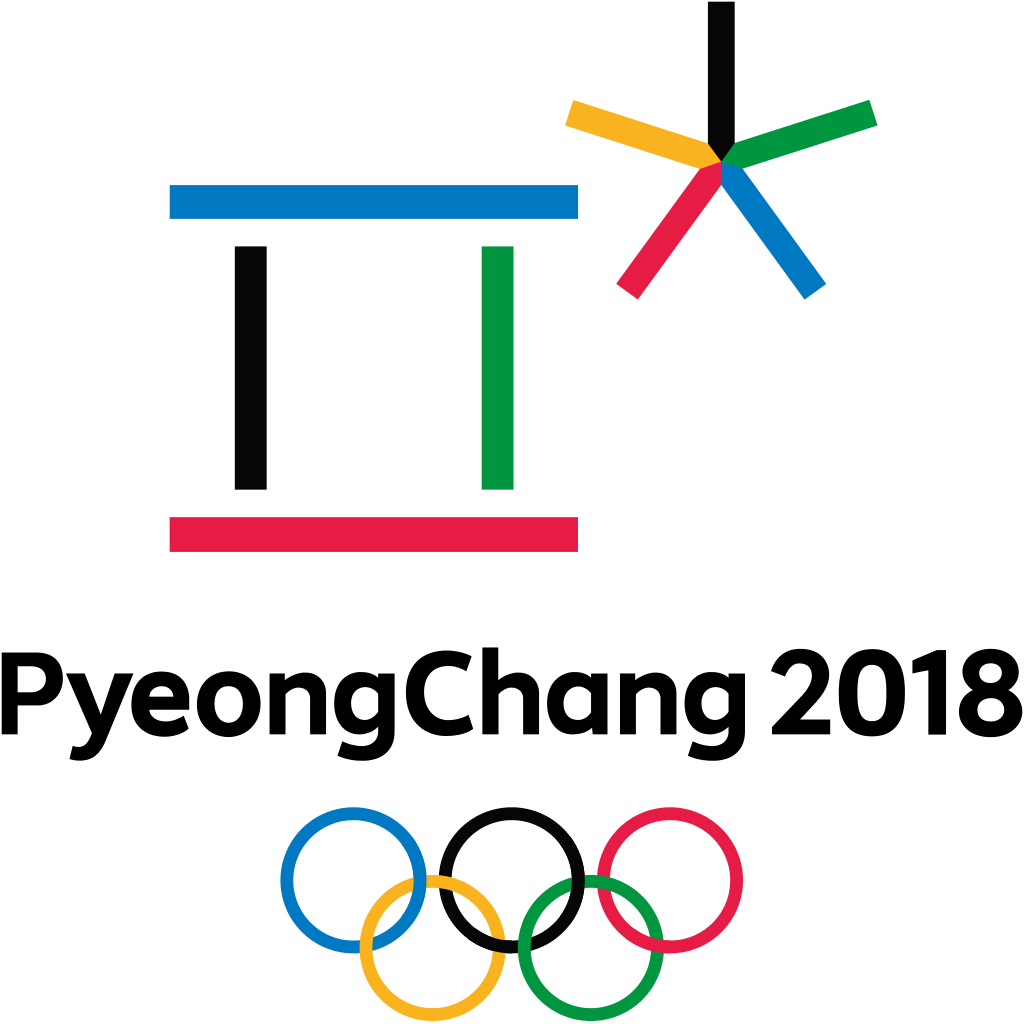
\includegraphics[width=0.7\textwidth]{Images/Olympics.png}
\end{frame}

\end{document}
